%%%%%%%%%%%%%%%%%%%%%%%%%%%%%%%%%%%%%%%%%
% Homework Assignment Article
% LaTeX Template
% Version 1.3.1 (ECL) (08/08/17)
%
% This template has been downloaded from:
% Overleaf
% Original author:
% Victor Zimmermann (zimmermann@cl.uni-heidelberg.de)
%
% License:
% CC BY-SA 4.0 (https://creativecommons.org/licenses/by-sa/4.0/)
%
%%%%%%%%%%%%%%%%%%%%%%%%%%%%%%%%%%%%%%%%%

%----------------------------------------------------------------------------------------

\documentclass[a4paper]{article} % Uses article class in A4 format

%----------------------------------------------------------------------------------------
%	FORMATTING
%----------------------------------------------------------------------------------------

\addtolength{\hoffset}{-2.25cm}
\addtolength{\textwidth}{4.5cm}
\addtolength{\voffset}{-3.25cm}
\addtolength{\textheight}{5cm}
\setlength{\parskip}{0pt}
\setlength{\parindent}{0in}

%----------------------------------------------------------------------------------------
%	PACKAGES AND OTHER DOCUMENT CONFIGURATIONS
%----------------------------------------------------------------------------------------

\usepackage{blindtext} % Package to generate dummy text
% \usepackage[style=numeric,sorting=none]{biblatex}
\usepackage{charter} % Use the Charter font
\usepackage[utf8]{inputenc} % Use UTF-8 encoding
\usepackage{microtype} % Slightly tweak font spacing for aesthetics

\usepackage[english]{babel} % Language hyphenation and typographical rules

\usepackage{amsthm, amsmath, amssymb} % Mathematical typesetting
\usepackage{float} % Improved interface for floating objects
\usepackage[export]{adjustbox}
\usepackage{wrapfig}
\usepackage[final, colorlinks = true, 
            linkcolor = black, 
            citecolor = black]{hyperref} % For hyperlinks in the PDF
\usepackage{graphicx, multicol} % Enhanced support for graphics
\graphicspath{ {./images/} }
\usepackage{xcolor} % Driver-independent color extensions
\usepackage{marvosym, wasysym} % More symbols
\usepackage{rotating} % Rotation tools
\usepackage{censor} % Facilities for controlling restricted text
\usepackage{listings, style/lstlisting} % Environment for non-formatted code, !uses style file!
\usepackage{pseudocode} % Environment for specifying algorithms in a natural way
\usepackage{style/avm} % Environment for f-structures, !uses style file!
\usepackage{booktabs} % Enhances quality of tables

\usepackage{tikz-qtree} % Easy tree drawing tool
\tikzset{every tree node/.style={align=center,anchor=north},
         level distance=2cm} % Configuration for q-trees
\usepackage{style/btree} % Configuration for b-trees and b+-trees, !uses style file!

% \usepackage[backend=biber,style=numeric,
            % sorting=nyt]{biblatex} % Complete reimplementation of bibliographic facilities
% \addbibresource{ecl.bib}
\usepackage{csquotes} % Context sensitive quotation facilities

\usepackage[yyyymmdd]{datetime} % Uses YEAR-MONTH-DAY format for dates
\renewcommand{\dateseparator}{-} % Sets dateseparator to '-'

\usepackage{fancyhdr} % Headers and footers
\pagestyle{fancy} % All pages have headers and footers
\fancyhead{}\renewcommand{\headrulewidth}{0pt} % Blank out the default header
\fancyfoot[L]{School of Computing, Macquarie University} % Custom footer text
\fancyfoot[C]{} % Custom footer text
\fancyfoot[R]{\thepage} % Custom footer text

\usepackage{comment}
\newcommand{\note}[1]{\marginpar{\scriptsize \textcolor{red}{#1}}} % Enables comments in red on margin

%----------------------------------------------------------------------------------------

\begin{document}

%----------------------------------------------------------------------------------------
%	TITLE SECTION
%----------------------------------------------------------------------------------------

\title{COMP3100 project report} % Article title
\fancyhead[C]{}
\hrule \medskip % Upper rule
\begin{minipage}{1\textwidth} % Center of title section
\centering 
\large % Title text size
Project report: Stage 1\\ % Assignment title and number
COMP3100 Distributed Systems, S1, 2023\\
\normalsize % Subtitle text size
SID: 45904979, Name: Lewis McCarthy
%%%%\\ % Assignment subtitle
\end{minipage}
\medskip\hrule % Lower rule
\bigskip

%----------------------------------------------------------------------------------------
%	ARTICLE CONTENTS
%----------------------------------------------------------------------------------------
\section{Introduction}
The COMP3100 Distributed Systems scheduling project involves re-implementing the client-side simulator for \texttt{ds-sim}\cite{ds-sim}, a distributed systems simulator designed to be language-independent. In stage 1 of the project, we were tasked with implementing the basic functionality required for the client to work, which included:
\begin{itemize}
	\item Connecting to the server
	\item Handshaking with the server
	\item Recieving and scheduling jobs
	\item Correctly quitting and disconnecting from the server 
 \end{itemize}

To schedule jobs, we had to implement a job scheduler known as Largest-Round-Robin (LRR), "that sends each job to a server of
the largest type in a round-robin fashion"\cite{assignment-stage-1-spec}. If multiple server types have the same number of cores, we proceed with the first server type listed.

The client-side simulator was to be programmed in the Java programming language, although the language of choice was seemed to be negotiable as long as it was readable, and it was to be delivered on GitHub\cite{assignment-git} by the due date on the 3rd of April 2023.
\section{System Overview}

\begin{wrapfigure}{rh}{0.5\textwidth}
	\centering
	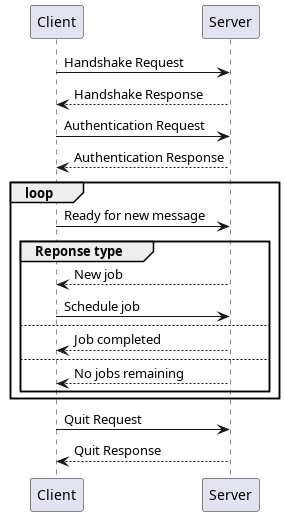
\includegraphics[width=0.35\textwidth]{sequence}
	\caption{Sequence diagram of the system}
\end{wrapfigure}

\sloppy
\subsection{Server}
The server-side program is responsible for simulating a distributed system based on a configuration file provided to it via arguments. The server generates jobs to simulate requests, and these jobs are then sent to the client to be scheduled. Upon the completion of a simulated job, the server will send the client a completed job message. Upon the total completion of job scheduling and when all jobs are done, the server will send a final message of \texttt{NONE}.

\subsection{Client}
\sloppy
The client-side program is responsible for establishing and authorizing a connection with the server, receiving jobs from the server, and scheduling these jobs based on the available servers. The client's main function is to schedule the provided jobs in such a way that it can make the best use of available resources. For stage 1, the client is only required to have the LRR scheduler implemented. This scheduler sends each job to a server of the largest type in a round-robin fashion. For example, with 3 largest servers, the order would be: Largest 1, Largest 2, Largest 3, Largest 1, etc.
\vfil \break

\clearpage
\section{Design}

\subsection{Philosophy}
I designed the client-side simulator to be as simple and future-proof as possible. I wanted to be able to program a working solution fairly quickly, so I structured it around giving each method a specific, singular function it would perform. I did not hold myself too strictly to this, but enough that this approach would probably be clear to any reader.
For future-proofing, I made sure that I would be able to easily update the code to account for different schedulers in the future. I based this on the information and short summary provided for the 2nd stage of the project.

\subsection{Considerations}
As this is an assignment, the implementation needs to be clear and quickly understandable for the purposes of marking. It also needed to be written in a way that I would be able to easily explain its functionality and structure weeks later. To achieve this, I wrote it in such a way that the primary steps the client goes through are clear in the main function, while the code doing the actual work is above in the Client class. \\
I also made the decision to omit launch arguments. While generally it's a good idea and it would fall in line with future-proofing, I didn't feel compelled to add it at the current time. This was primarily due to the current limited functionality of the program, but it also meant one less process to debug.

\subsection{Functionality}

When actually designing the system, I followed the design suggested by the provided pseudocode fairly closely. This resulted in a fairly straightforward design that worked almost straight away.

\begin{figure}[H]
	\centering
	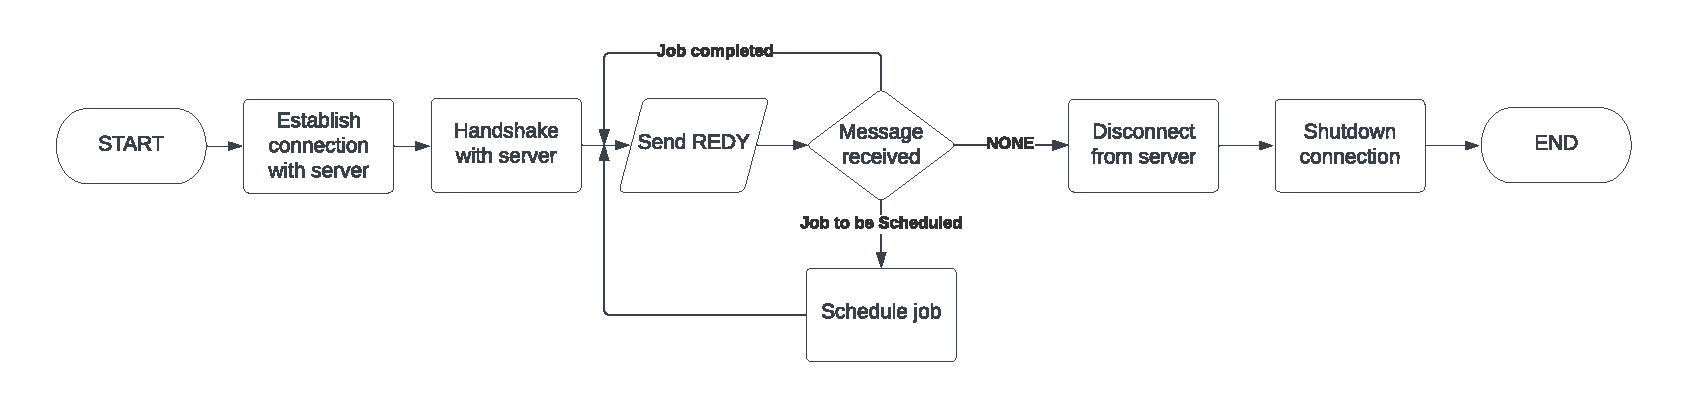
\includegraphics[width=1.0\textwidth]{flowchart}
	\caption{High level flowchart of Client program}
\end{figure}

The primary steps taken by the client are as follows:
\begin{itemize}
	\item \textbf{Establish connection with server}: This is the first action taken by the client where the socket connection is established.
	\item\textbf{Handshake with server}: The handshake is performed, and a username is used to authorize the connection.
	\item\textbf{Send REDY}: The client sends a message to the server indicating that it is ready to receive a new message.
	\item\textbf{Message recieved}: A decision is made depending on the message received. If a new job message is received, it is scheduled using the LRR scheduler. A job completed message is currently ignored, and a "none" message starts the disconnection process.
	\item\textbf{Schedule job}: The job received is taken and scheduled using the LRR scheduler. Within this process, a request is sent to the server to return servers capable of handling the job to be scheduled.
	\item\textbf{Disconnect from server}: The client sends an exit message and waits for the response.
	\item\textbf{Shutdown connection}: The socket connection is closed.
\end{itemize}
\section{Implementation}

\subsection{Technology}
The client was written in Java with no addition non-default libraries, except for the ArrayList class which is part of the Java standard library.
For quickly building and testing the program, I created a Makefile that allows for quick compilation and testing of the program. By default, the Makefile compiles and runs the program, but I also provided options to perform these tasks individually and one for testing using the provided test files.

\subsection{Data structures}
\begin{itemize}
	\item  \texttt{DSClient}: The main class that the program was written and everything else interacts with
	\item  \texttt{ServerJob}: This is a basic struct-like class mostly for the purpose of clean code used to store the data of a given job.
	\item  \texttt{ServerListEntry}: Another struct-like class also for the purpose of clean code. But also used inconjunction with the \texttt{ArrayList} class to store the servers that the simulated server had returned.
\end{itemize}

\subsection{Methods}
The DSClient class contains several public, private and helper methods that implement the functionalities of the client. \\
The public methods are:
\begin{itemize}
	\item  \texttt{connect()}: Establishes a TCP/IP socket connection to the server.
	\item \texttt{connection\_handshake()}: Performs the handshake with the server and authenticates the user.
	\item \texttt{schedule\_job(String, AlgorthimType)}: Schedules a job given by a \texttt{JOBN} message and a given algorthim type enum.
	\item \texttt{disconnect()}: Sends the \texttt{EXIT} message to the server and waits for the reply.
	\item \texttt{shutdown()}: Closes the data output stream and TCP/IP socket.
\end{itemize}

The private methods are:
\begin{itemize}
	\item \texttt{find\_capable\_servers(ServerJob)}: Sends a \texttt{GETS} command to the server to request information about available servers that can run the given job.
	\item  \texttt{get\_server(AlgorthimType)}: Gets the best fitting server based on the AlgorthimType enum argument parsed. Currently the only enum is \texttt{ALG\_LRR}.
	\item  \texttt{get\_server\_lrr()}: Finds the best fitting server using the LRR scheduler. 
\end{itemize}

There are also a few helper methods which are:
\begin{itemize}
	\item  \texttt{send\_and\_wait(String)}: Takes the String argument parsed and sends it to the server. After which it waits for the response and returns the first line recieved.
	\item  \texttt{error\_mismatch(String, String)}: Basically a C-style macro for printing out if an message doesn't match what it's supposed to. Used in the handshake and disconnect methods.
\end{itemize}
%----------------------------------------------------------------------------------------
%	REFERENCE LIST
%----------------------------------------------------------------------------------------
\bibliographystyle{ieeetr}
\bibliography{comp3100project}
% \printbibliography

%----------------------------------------------------------------------------------------

\end{document}
